% -*- coding: UTF-8 -*-
\documentclass{article}
\usepackage{amsmath}
\usepackage{tikz}

\begin{document}
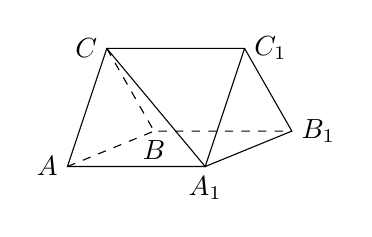
\begin{tikzpicture}

  \coordinate[label=180:$A$] (a) at (0,0);
  \coordinate[label=-90:$B$] (b) at (0.6+0.5,0.45);
  \coordinate[label=180:$C$] (c) at (0.5,1.5);
  \coordinate[label=-90:$A_1$] (d) at (1.75,0);
  \coordinate[label=0:$B_1$] (e) at (2.35+0.5,0.45);
  \coordinate[label=0:$C_1$] (f) at (2.25,1.5);

  \draw (c) -- (a) -- (d) -- (e) -- (f) -- cycle -- (d) -- (f);
  \draw[dashed] (a) -- (b) (c) -- (b) -- (e);

\end{tikzpicture}
\end{document}
